\documentclass{beamer}
\mode<presentation>
\usepackage{amsmath,amssymb,mathtools}
\usepackage{textcomp}
\usepackage{gensymb}
\usepackage{adjustbox}
\usepackage{subcaption}
\usepackage{enumitem}
\usepackage{multicol}
\usepackage{listings}
\usepackage{url}
\usepackage{graphicx} % <-- needed for images
\def\UrlBreaks{\do\/\do-}

\usetheme{Boadilla}
\usecolortheme{lily}
\setbeamertemplate{footline}{
  \leavevmode%
  \hbox{%
  \begin{beamercolorbox}[wd=\paperwidth,ht=2ex,dp=1ex,right]{author in head/foot}%
    \insertframenumber{} / \inserttotalframenumber\hspace*{2ex}
  \end{beamercolorbox}}%
  \vskip0pt%
}
\setbeamertemplate{navigation symbols}{}

\lstset{
  frame=single,
  breaklines=true,
  columns=fullflexible,
  basicstyle=\ttfamily\tiny   % tiny font so code fits
}

\numberwithin{equation}{section}

% ---- your macros ----
\providecommand{\nCr}[2]{\,^{#1}C_{#2}}
\providecommand{\nPr}[2]{\,^{#1}P_{#2}}
\providecommand{\mbf}{\mathbf}
\providecommand{\pr}[1]{\ensuremath{\Pr\left(#1\right)}}
\providecommand{\qfunc}[1]{\ensuremath{Q\left(#1\right)}}
\providecommand{\sbrak}[1]{\ensuremath{{}\left[#1\right]}}
\providecommand{\lsbrak}[1]{\ensuremath{{}\left[#1\right.}}
\providecommand{\rsbrak}[1]{\ensuremath{\left.#1\right]}}
\providecommand{\brak}[1]{\ensuremath{\left(#1\right)}}
\providecommand{\lbrak}[1]{\ensuremath{\left(#1\right.}}
\providecommand{\rbrak}[1]{\ensuremath{\left.#1\right)}}
\providecommand{\cbrak}[1]{\ensuremath{\left\{#1\right\}}}
\providecommand{\lcbrak}[1]{\ensuremath{\left\{#1\right.}}
\providecommand{\rcbrak}[1]{\ensuremath{\left.#1\right\}}}
\theoremstyle{remark}
\newtheorem{rem}{Remark}
\newcommand{\sgn}{\mathop{\mathrm{sgn}}}
\providecommand{\abs}[1]{\left\vert#1\right\vert}
\providecommand{\res}[1]{\Res\displaylimits_{#1}}
\providecommand{\norm}[1]{\lVert#1\rVert}
\providecommand{\mtx}[1]{\mathbf{#1}}
\providecommand{\mean}[1]{E\left[ #1 \right]}
\providecommand{\fourier}{\overset{\mathcal{F}}{ \rightleftharpoons}}
\providecommand{\system}{\overset{\mathcal{H}}{ \longleftrightarrow}}
\providecommand{\dec}[2]{\ensuremath{\overset{#1}{\underset{#2}{\gtrless}}}}
\newcommand{\myvec}[1]{\ensuremath{\begin{pmatrix}#1\end{pmatrix}}}
\newcommand{\mydet}[1]{\ensuremath{\begin{vmatrix}#1\end{vmatrix}}}

\newenvironment{amatrix}[1]{%
  \left(\begin{array}{@{}*{#1}{c}|*{#1}{c}@{}}
}{%
  \end{array}\right)
}

\newcommand{\myaugvec}[2]{\ensuremath{\begin{amatrix}{#1}#2\end{amatrix}}}
\let\vec\mathbf
% ---------------------

\title{Matgeo Presentation - Problem 9.6.5}
\author{ee25btech11056 - Suraj.N}

\begin{document}

\begin{frame}
  \titlepage
\end{frame}

\begin{frame}{Problem Statement}

Solve
\[
\frac{1}{3x+y} + \frac{1}{3x-y} = \frac{3}{4}, \quad 
\frac{1}{2(3x+y)} - \frac{1}{2(3x-y)} = -\frac{1}{8}.
\]

\end{frame}

\begin{frame}{Data}

\begin{table}[h!]
  \centering
  \begin{tabular}{|c|c|}
\hline
\textbf{Name} & \textbf{Value} \\ \hline
$\vec{A}$ & $\myvec{2 & 1 \\0 & 3}$ \\ \hline
\end{tabular}

  \caption*{Table : Hyperbola}
  \label{9.6.5}
\end{table}

\end{frame}

\begin{frame}{Solution}

By rearranging the two equations we get the equation of two hyperbolas as :

\begin{align}
  9x^2 - y^2 -8y &= 0\\
  9x^2 - y^2 -8x &= 0
\end{align}

The conic parameters for the two hyperbolas can be expressed as :

\begin{align}
  \vec{V_1} &= \myvec{9 & 0\\0 & -1} & \vec{u_1} &= \myvec{0 \\ -4} & f1 &= 0\\
  \vec{V_2} &= \myvec{9 & 0\\0 & -1} & \vec{u_2} &= \myvec{-4 \\ 0} & f2 &= 0
\end{align}

The intersection of two conics is defined as :

\begin{align}
  \vec{x}^\top(\vec{V_1}+\mu\vec{V_2})\vec{x} + 2(\vec{u_1}+\mu\vec{u_2})^\top\vec{x} + (f1 + \mu f2) = 0 \label{eq:conic} 
\end{align}

\end{frame}

\begin{frame}{Solution}

The above equation represents a pair of straight lines if :

\begin{align}
  \mydet{\vec{V_1}+\mu\vec{V_2} & \vec{u_1}+\mu\vec{u_2}\\(\vec{u_1}+\mu\vec{u_2})^\top & f1 + \mu f2} &= 0
\end{align}

Substituting the values in the above equation :

\begin{align}
  \mydet{9+9\mu & 0 & -4\mu\\0 & -1-\mu & -4\\-4\mu & -4 & 0} &= 0
\end{align}

\end{frame}

\begin{frame}{Solution}

Applyint row reduction to find determinant:

\begin{align}
\mydet{9+9\mu & 0 & -4\mu\\0 & -1-\mu & -4\\-4\mu & -4 & 0} 
\xleftrightarrow{R_3 \to R_3 +\tfrac{4\mu}{9+9\mu}R_1}
\mydet{9+9\mu & 0 & -4\mu\\0 & -1-\mu & -4\\0 & -4 & -\tfrac{16\mu^2}{9+9\mu}}\\
\xleftrightarrow{R_3 \to R_3 -\tfrac{4}{1+\mu}R_2}
\mydet{9+9\mu & 0 & -4\mu\\0 & -1-\mu & -4\\0 & 0 & \tfrac{-16\mu^2+144}{9+9\mu}}
\end{align}

By finding the determinant we get 

\begin{align}
  (1+\mu)(-16\mu^2 + 144) &= 0\\
  \mu = -1 , \mu = \pm3
\end{align}

\end{frame}

\begin{frame}{Solution}

Substituting $\mu = -1$ in \eqref{eq:conic} we get equation of line as :

\begin{align}
  2\myvec{4 \\-4}^\top\vec{x} &= 0\\
  \myvec{-1 & 1}\vec{x} &= 0
\end{align}

The parameters of the line are :

\begin{align}
  \vec{h} &= \myvec{0\\0} & \vec{m} &= \myvec{1\\1}
\end{align}

Substituting the parameters of line and the first hyperbola in the below equation :
\begin{align}
\kappa_i
  &= \frac{1}{\vec{m}^\top \vec{V_1}\vec{m}}
     \left(
       -\,\vec{m}^\top\big(\vec{V_1}\vec{h}+\vec{u_1}\big)
       \;\pm\;
       \sqrt{ \big[\vec{m}^\top(\vec{V_1}\vec{h}+\vec{u_1})\big]^2
       - g(\vec{h})\,\big(\vec{m}^\top \vec{V_1}\vec{m}\big)}
     \right)\\
  \kappa_i &= 0,1
\end{align}

\end{frame}

\begin{frame}{Solution}

Therefore the points of intersections of the line and first hyperbola are :

\begin{align}
  \vec{P_1}&=\myvec{1\\1} & \vec{P_2} = \myvec{0\\0}
\end{align}

But if we substiture $\vec{P_2}$ in the original equation we get 0 in the denominator , which is undefined.\\
Therefore the solution for the given equations is :

\begin{align}
  \vec{P} &= \myvec{1\\1}
\end{align}

\end{frame}

\begin{frame}{Plot}

\begin{figure}[h!]
  \centering
  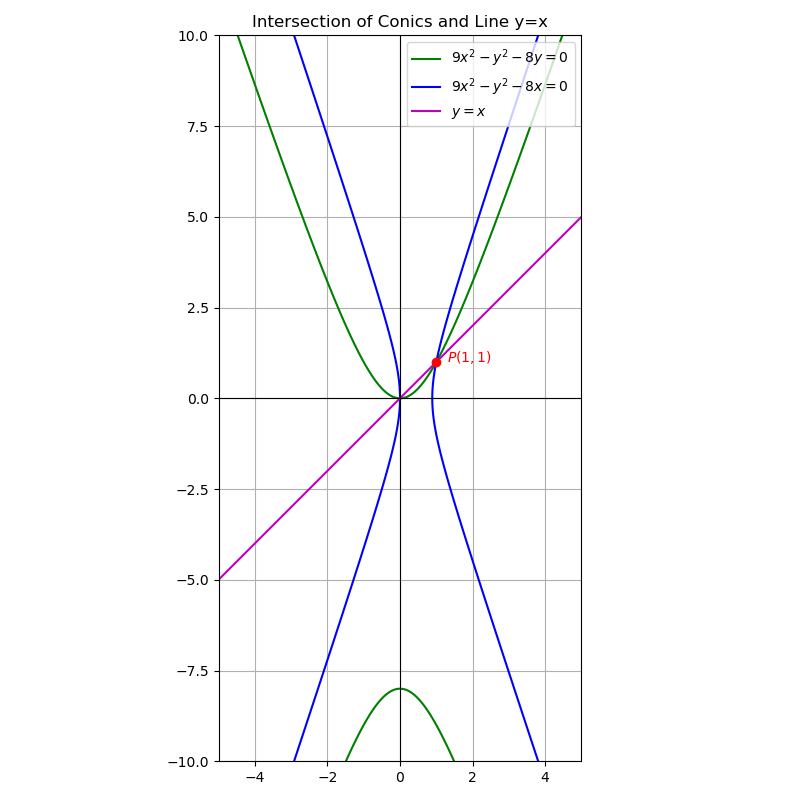
\includegraphics[width=0.6\columnwidth]{figs/conics_intersection.png} 
   \caption*{Fig : Hyperbola and Line}
  \label{Fig1}
\end{figure}

\end{frame}

\end{document}

